\documentclass[serif,8pt]{beamer}
\usepackage{beamerthemeshadow}
\usepackage{textcomp}
\usepackage[spanish]{babel}
\usepackage[utf8]{inputenc}
\usepackage{listings}
\usetheme{Warsaw}

\logo{
\includegraphics[scale=0.1]{./img/debianday.png}}
\begin{document}
\title[\textbf{Debian Day -- 2015}] {SELinux }
\subtitle{Security Enhanced Linux}
\author[Gonzalo Nina Mamani]{  Gonzalo Nina Mamani \\ gonzalo@hiperborea.com.bo}
\date{ \textbf{Debian Day - Cochabamba } \\ \textcopyleft Copyleft  2015 \\ Reproducción permitida bajo los terminos de la licencia de documentación libre GNU} 

\frame{\titlepage} 

\frame{\frametitle{Contenido}\tableofcontents} 


\section{Presentación} 
\subsection{Acerca de mi}
\frame{\frametitle{¿Quien esta aqui delante?} 
\begin{columns}
  	\column{.5\textwidth} 
		
\includegraphics[scale=.5]{./img/yo2.jpg} 
  	\column{.65\textwidth}
  	\begin{itemize}
  	  \item Gonzalo Nina Mamani.
  	  \item Director Area Seguridad en \textbf{Hiperborea IT Security}.
  	  \item Fedora Ambassadors Bolivia.\\ {\tiny lorddemon@fedoraproject.org}
  	  \item Linux user from 2008.\\ \textbf{Started with Debian.}
  	  \vspace{1cm} 
  	  \item Correo: \textit{gonzalo@hiperborea.com.bo} \\ Twitter: \textit{@lorddemon} \\ Facebook: \textit{www.fb.com/gonzalon}
  	\end{itemize}
 	\end{columns}

}
\subsection{Seguridad Informática y GNU/Linux}
\frame{ 
\begin{center}
¿Como relacionamos la seguridad informática y GNU/Linux?\\
  
\includegraphics[scale=0.3]{./img/tuxp.jpeg} 
\end{center}
}

\section{Security Enhanced Linux} 
\subsection{Nociones Basicas}
\frame{\frametitle{Mandatory Access Control}
\begin{columns}
  \column{.4\textwidth}
  “Mandatory Access Control” o MAC, añade la posibilidad de limitar, denegar, a cualquier sujeto, la posibilidad de iniciar procesos, subprocesos, o en general, el acceso a recursos:
  \begin{itemize}
    \item Archivos
    \item Directorios
    \item Bloques de memoria
    \item puertos TCP/UDP, entre otros.
  \end{itemize} 
  \column{.5\textwidth}
  Operan a nivel del núcleo, por ejemplo, acceder a la red vía un puerto específico, una regla en el propio núcleo le permitirá consultar si ese recurso está disponible para ese servicio.

En GNU/Linux hay al menos 4 MAC conocidos:

\begin{itemize}
  \item Tomoyo Linux
  \item GRSecurity
  \item AppArmor
  \item SELinux
\end{itemize}
\end{columns}
}

\frame{\frametitle{SELinux Securiy Enhanced Linux}
\begin{block}{SELinux Securiy Enhanced Linux}
SELinux (Security Enhanced Linux) es uno de los proyectos de un MAC Security Linux más antiguos, SELinux basa sus reglas en tratar “todo elemento” como un objeto, luego, etiquetarlo con permisos que puedan ser entendidos por el núcleo, los procesos son etiquetados y corren cada uno en su propio dominio. Así, se pueden definir reglas de cómo un dominio interactua con los otros, permitiendo un control granular en la seguridad.
\end{block}
}

\subsection{Type Enforcement }
\frame{\frametitle{Tipos de procesos}
\begin{center}
    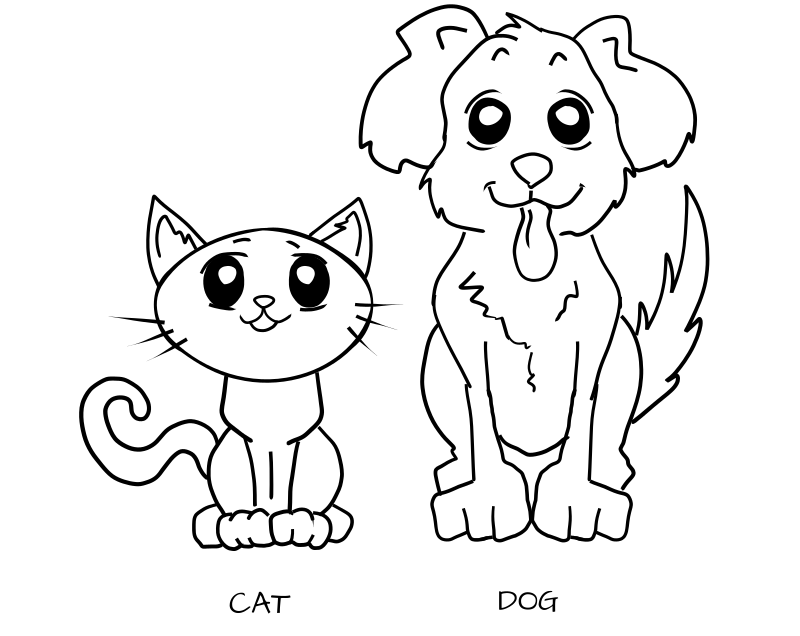
\includegraphics[scale=0.3]{./img/1.png} 
  \end{center}
}
\frame{\frametitle{Tipos de Objetos}
\begin{center}
    
\includegraphics[scale=0.3]{./img/2.png}
  \end{center} 
}
\frame{\frametitle{Politicas por Reglas}
\begin{center}
    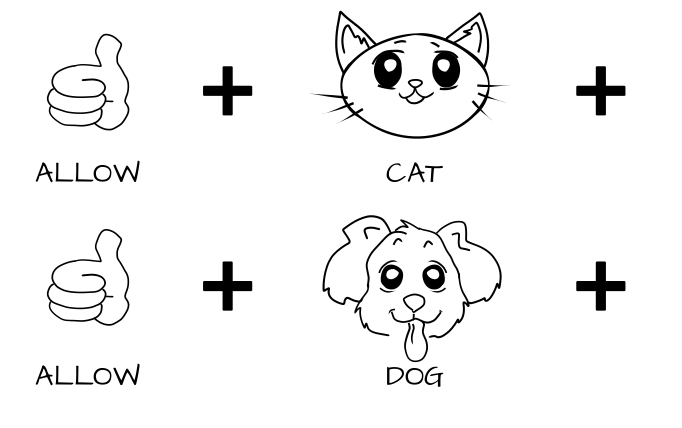
\includegraphics[scale=0.3]{./img/3.png} 
  \end{center}
}
\frame{\frametitle{Politicas por Reglas}
\begin{center}
    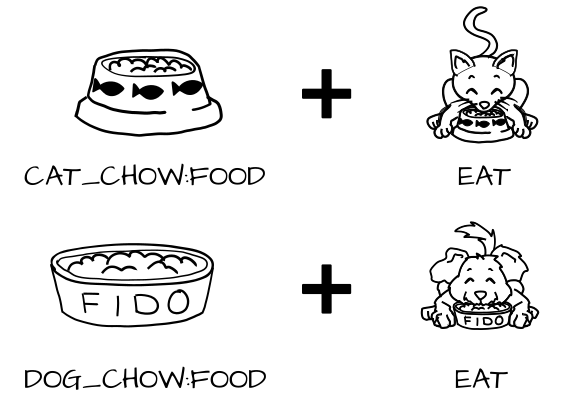
\includegraphics[scale=0.3]{./img/4.png} 
  \end{center}
}
\frame{\frametitle{Yummy Yummy}
  
\includegraphics[scale=0.3]{./img/5.png} 
    
\includegraphics[scale=0.3]{./img/6.png} 
}
\frame{\frametitle{Perro Malo}
\begin{center}
    
\includegraphics[scale=0.3]{./img/7.png} 
  \end{center}
}
\frame{\frametitle{Gato Malo}
\begin{center}
    
\includegraphics[scale=0.3]{./img/8.png} 
  \end{center}
}
\subsection{MCS Enforcement }
\frame{\frametitle{Multi Category Security MCS}
\begin{center}
    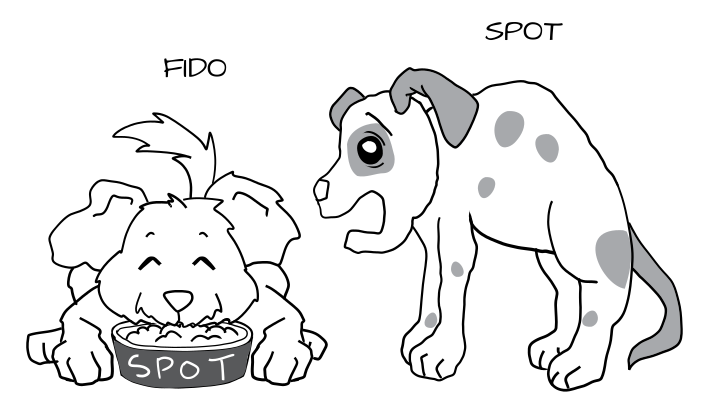
\includegraphics[scale=0.3]{./img/9.png} 
  \end{center}
}
\frame{\frametitle{Multi Category Security MCS}
\begin{center}
    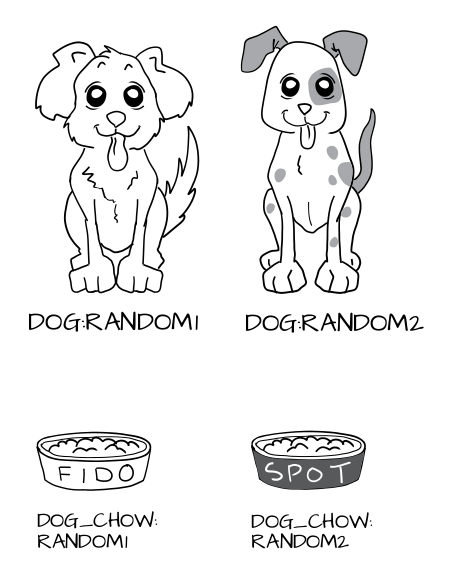
\includegraphics[scale=0.3]{./img/10.png} 
  \end{center}
}
\frame{\frametitle{Type Enforcement}
\begin{center}
    
\includegraphics[scale=0.3]{./img/11.png} 
  \end{center}
}
\frame{\frametitle{Multi Category Security Enforcement}
\begin{center}
    
\includegraphics[scale=0.3]{./img/12.png} 
  \end{center}
}
\frame{\frametitle{Contextos de seguridad y usuarios Unix}
\begin{center}
    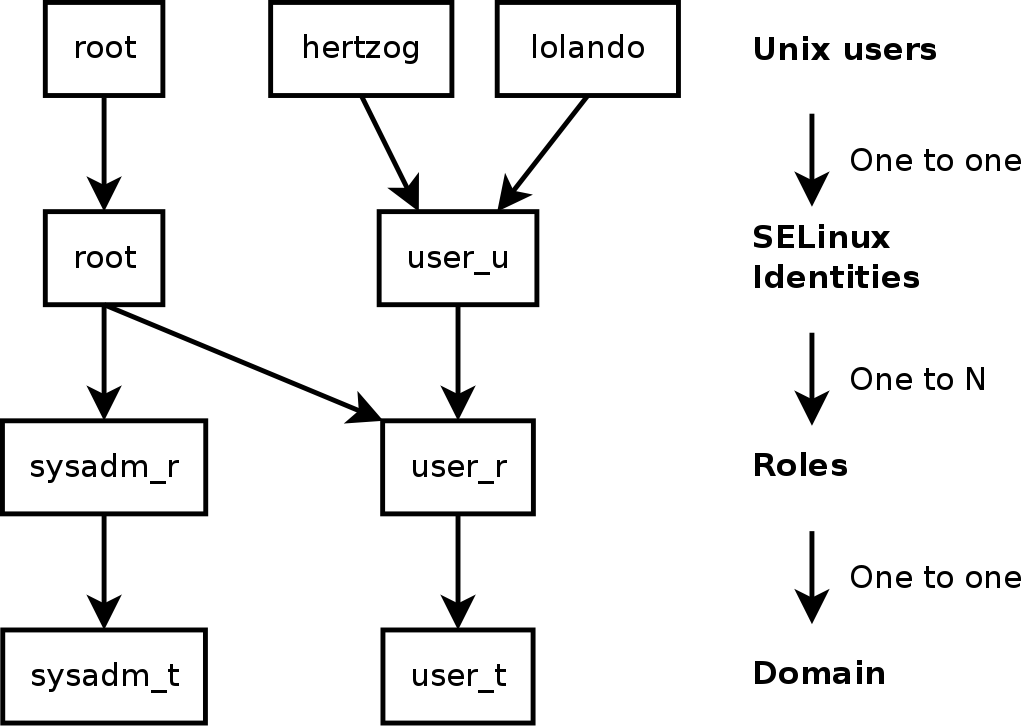
\includegraphics[scale=0.3]{./img/p1.png} 
  \end{center}
}
\frame{\frametitle{Transiciones automáticas entre dominios}
\begin{center}
    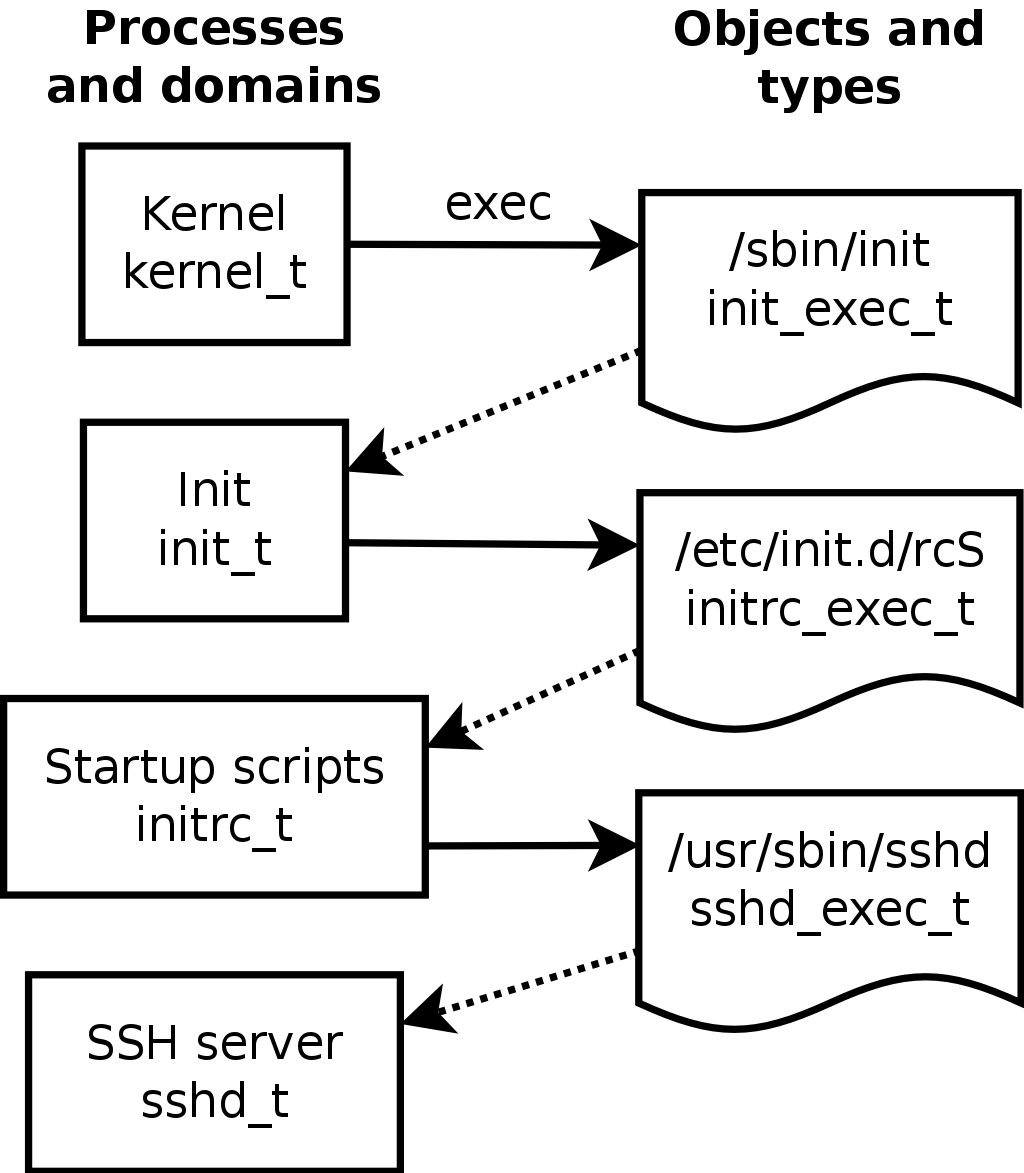
\includegraphics[scale=0.3]{./img/p2.png} 
  \end{center}
}


\section{Demostración Practica} 
\subsection{Contexto de seguridad}
\frame{\frametitle{Averiguar el contexto de seguridad}
\begin{block}{Averiguar el contexto de seguridad}
Para averiguar el contexto de seguridad de un proceso
\begin{itemize}
  \item ps -axZ
\end{itemize}

Para averiguar el contexto de seguridad em una consola
\begin{itemize}
  \item id -Z
\end{itemize}

Por último, para averiguar el tipo asignado a un archivo
\begin{itemize}
  \item ls -Z /usr/bin/ssh
\end{itemize}


\end{block}

}
\section{Referencias}
\begin{frame}\frametitle<presentation>{Referencias}
	\begin{thebibliography}{10}
	      \bibitem{Debian Asegurando Rapidamente Con SELinux}
        Debian Asegurando Rapidamente Con SELinux
	      \newblock 
	      \href{http://blog.phenobarbital.info/2013/07/debian-asegurando-rapidamente-con-selinux/}{http://blog.phenobarbital.info/2013/07/debian-asegurando-rapidamente-con-selinux/}

	      \bibitem[El libro del administrador de Debian]{El libro del administrador de Debian}
		El libro del administrador de Debian
	      \newblock {\em Seccion 14.4. Introducción a SELinux}
	      \newblock 
	      \href{https://debian-handbook.info/browse/es-ES/stable/sect.selinux.html}{https://debian-handbook.info/browse/es-ES/stable/sect.selinux.html}

	      \bibitem{The SELinux Coloring Book} 
	      The SELinux Coloring Book
	      \newblock {\em Un libro interesante para entender SELinux}.
	      \newblock 
	      \href{https://people.redhat.com/duffy/selinux/selinux-coloring-book\_A4-Stapled.pdf}{https://people.redhat.com/duffy/selinux/selinux-coloring-book\_A4-Stapled.pdf}

	      
	\end{thebibliography}
    \end{frame}
\end{document}
